\documentclass[a4paper]{article}

% Language and font encodings
\usepackage[english]{babel}
\usepackage[a4paper,top=3cm,bottom=2cm,left=3cm,right=3cm,marginparwidth=1.75cm]{geometry}
\usepackage{amsmath}
\usepackage{graphicx}
\usepackage{tabularx}
\usepackage{natbib}
\usepackage{subcaption}
\usepackage[colorinlistoftodos]{todonotes}
\usepackage[colorlinks=true, allcolors=blue]{hyperref}
\usepackage{wrapfig}
\DeclareMathAlphabet{\pazocal}{OMS}{zplm}{m}{n}
\usepackage{setspace}
\usepackage{hyperref}
\hypersetup{
    colorlinks=true,
    linkcolor=blue,
    filecolor=magenta,      
    urlcolor=cyan,
}
\urlstyle{same}

%%%%%%%%%%%%%%%%%%%%%%%%%%%%%%%%%%%%%%%%%%%%%%%%%%%%%%%%%%%%%%%%%%%%%%%%%%%%%%%%

\begin{document}

\begin{center}
  {\Large \bf Milestone 3: The Evolution of Structures in the Universe.}\\[4ex]
  {\large Daniel Herman}\\[4ex]
  \normalsize
  \today
  \vspace*{8ex}
      
  \begin{minipage}[t]{12cm}
      
  {\bf Abstract.} Calculating the evolution of density perturbations and velocity distributions of dark matter and baryonic matter. We also calculate the evolution of the first six moments of the photon perturbations and the physical potentials $\Phi$ and $\Psi$.
	
  \vspace*{8ex}
  \end{minipage}

\end{center}

\section{Introduction}\label{sec:intro}

In this milestone we utilize the infrastructure that was created in the first two milestones to calculate and visualize the behavior of perturbations from the early universe onwards.\\

Specifically, in this milestone we make some specific caluclations before recombination during an era where the photons are tightly coupled to the baryons, which we call tight coupling. Using results from Milestone 2 allow us to determine the era of tight coupling by looking at the optical depth $\tau$, and therefore the electron density of the universe.\\

The main focus of this milestone is to compute a two dimensional grid of physical quantities in time, $x$, and Fourier scale, $k$. In order to calculate these fully, we also need to calculate their derivatives. These specific quantities are $\Phi(x,k), \Psi(x,k), \delta(x,k), \delta_b(x,k), v(x,k), v_b(x,k),$ and $\Theta_l(x,k)$.\\

In a similar fashion to the first two milestones we utilize provided skeleton code and an ODE solver to calculate the desired quantities. All calculations are performed using FORTRAN 90, and all plots are created using Python.

\clearpage

\section{Equations}\label{sec:label}
Over the last two months of lecture, we have derived the Einstein-Boltzmann equations, which I will not include here. Seeing as these equations describe the evolution of perturbations, they all take the form of differential equations. This means for us, that in order to accurately calculate the values of the physical quantities in question we must calculate the values as well as their derivatives at each time step $x$. The solutions to the Einstein-Boltzmann equations can be found in section \ref{subsec:einbol}.

\subsection{Initial Conditions}\label{subsec:init}
To start our calculations, we must initialize the conditions for the universe. By inspecting the equations are their solutions, we see that all calculated physical quantities depend on the potential $\Phi$. For simplicity, we scale the equations by setting $\Phi_{initial} = 1$. The rest of the initial conditions are as follows:

\begin{align}
\Phi =& 1 \\
\delta =& \delta_b = \dfrac{3}{2}\Phi \\
v =& v_b = \dfrac{ck}{2\pazocal{H}} \Phi \\
\Theta_0 =& \dfrac{1}{2} \Phi \\
\Theta_1 =& -\dfrac{ck}{6\pazocal{H}} \Phi \\
\Theta_2 =& - \dfrac{20ck}{45\pazocal{H}\tau`} \Theta_1 \\
\Theta_l =& - \dfrac{l}{2l+1}\dfrac{ck}{\pazocal{H}\tau`} \Theta_{l-1}.
\end{align}


\subsection{Tight Coupling}\label{subsec:tight}

As mentioned in section \ref{sec:intro}, we have to make some adjustments to the solutions during tight coupling. The evolution of perturbations during tight coupling are very important to the state of the perturbations after recombination. The photons are tightly coupled to the baryons and therefore photon perturbations and baryon perturbations affect each other, as can be seen by the adjusted solutions. An important consequence of tight coupling is that higher moments of photon perturbations are supressed by the intertwined nature of this fluid. The tight coupling equations are listed here:

\begin{align}
q =& \dfrac{-[(1-2R)\tau' + (1+R)\tau''](3\Theta_1 + v_b) - \dfrac{ck}{\pazocal{H}}\Psi + (1-\dfrac{\pazocal{H}'}{\pazocal{H}})\dfrac{ck}{\pazocal{H}}(-\Theta_0 + 2\Theta_2) - \dfrac{ck}{\pazocal{H}}\Theta_0'}{(1+R)\tau'+ \dfrac{\pazocal{H}'}{\pazocal{H}}-1} \\
v_b' =& \dfrac{1}{1+R}\Big[-v_b - \dfrac{ck}{\pazocal{H}}\Psi + R(q + \dfrac{ck}{\pazocal{H}}(-\Theta_0 + 2\Theta_2) - \dfrac{ck}{\pazocal{H}}\Psi)\Big] \\
\Theta_1' =& \dfrac{1}{3}(q-v_b').
\end{align}

\subsection{Einstein-Boltzmann Equation Solutions}\label{subsec:einbol}

\begin{align}
\Theta_0' =& -\dfrac{ck}{\pazocal{H}}\Theta_1 - \Phi` \\
\Theta_1' =& \dfrac{ck}{3\pazocal{H}}\Theta_0 - \dfrac{2ck}{3\pazocal{H}}\Theta_2 + \dfrac{ck}{3\pazocal{H}}\Psi + \tau`\big[\Theta_1 + \dfrac{1}{3}v_b\big] \\
\Theta_l' =& \dfrac{lck}{(2l+1)\pazocal{H}}\Theta_{l-1} - \dfrac{(l+1)ck}{(2l1)\pazocal{H}}\Theta_{l+1} + \tau`\big[\Theta_l - \dfrac{1}{10}\Theta_l\delta{l,2}\big], 2 \leq l < l_{max} \\
\Theta_l' =& \dfrac{ck}{\pazocal{H}}\Theta_{l-1} - c\dfrac{l+1}{\pazocal{H}\eta(x)}\Theta_l + \tau`\Theta_l, l=l_{max} \\
\delta' =& \dfrac{ck}{\pazocal{H}}v - 3\Phi' \\
v' =& -v-\dfrac{ck}{\pazocal{H}}\Psi \\
\delta_b' =& \dfrac{ck}{\pazocal{H}}v_b - 3\Phi' \\
v_b' =& -v_b - \dfrac{ck}{\pazocal{H}}\Psi + \tau'R(3\Theta_1 + v_b) \\
\Phi' =& \Psi - \dfrac{c^2k^2}{3\pazocal{H}^2}\Phi + \dfrac{H_0^2}{2\pazocal{H}^2}[\Omega_m a^{-1}\delta + \Omega_b a^{-1} \delta_b + 4\Omega_r a^{-2}\Theta_0] \\
\Psi =& -\Phi- \dfrac{12H_0^2}{c^2k^2a^2}\Omega_r\Theta_2 \\
R  =& \dfrac{4\Omega_r}{3\Omega_ba}
\end{align}

\section{Implementaion}\label{sec:imp}

As mentioned in section \ref{subsec:init}, we simplify our calculations by setting $\Phi_{initial} = 1$ . We utilize the time and recombination modules which were created for Milestone 1 and Milestone 2 respectively, to assist in our calculations.  First, we initialize our perturbation equations by allocating arrays for the desired values and create a set of quadratic $k$ values that correspond to different scale sizes. For each of these $k$ values, we set the $\Phi, \Psi, \delta, \delta_b, v, v_b, \Theta_l$ initial conditions, which are the starting point for our calculations. \\

Once the quantities have been initialized, we begin integrating the derivatives of the physical quantities to calculate the approximate values at each time step. Before we can do this, we create a time-step grid. Since the perturbations are greatly influenced by the behavior before recombination, we create a grid of 1000 points between $x_{init}$ and $x_{start_rec}$ for higher resolution. A grid of 500 points is created for the following time, namely between $x_{start_rec}$ and $x_0 = 0$.\\

For our computation loop, we calculate all of the necessary physical quantities over the whole time grid, one $k$ value at a time (calculate everything for $k=1$, then $k=2$, etc.). To know when we need to use the tight coupling equations, we calculate the $x$ value for when tight coupling ends first. The criteria we use for this are such that the photons are tightly coupled when $\tau' > 10$ or $\dfrac{ck}{\pazocal{H}\tau'} < 0.1$. We also include the criteria that the photons cannot be coupled to the baryons after recombination has begun. \\

Since tight coupling supresses the higher moments of the photon perturbations, we only calculate the moments up to $\Theta_2$ during tight coupling, and set all higher moments to 0. Once tight coupling has ended, we solve for all moments $0 \leq l \leq l_{max} = 6$.\\

The results of our calculations are shown in the following section.

\section{Results}\label{sec:results}
In the following plots, the red tinted portion of the graph represents the era of recombination. The time where radiation and matter are equal $x_{eq}$ is also shown on the x-axis to help visualize the behavior of the perturbations and other physical quantities during the different epochs.

\begin{figure}[ht!]
\label{fig:delta}
\centering
\begin{minipage}{0.5\textwidth}
\centering
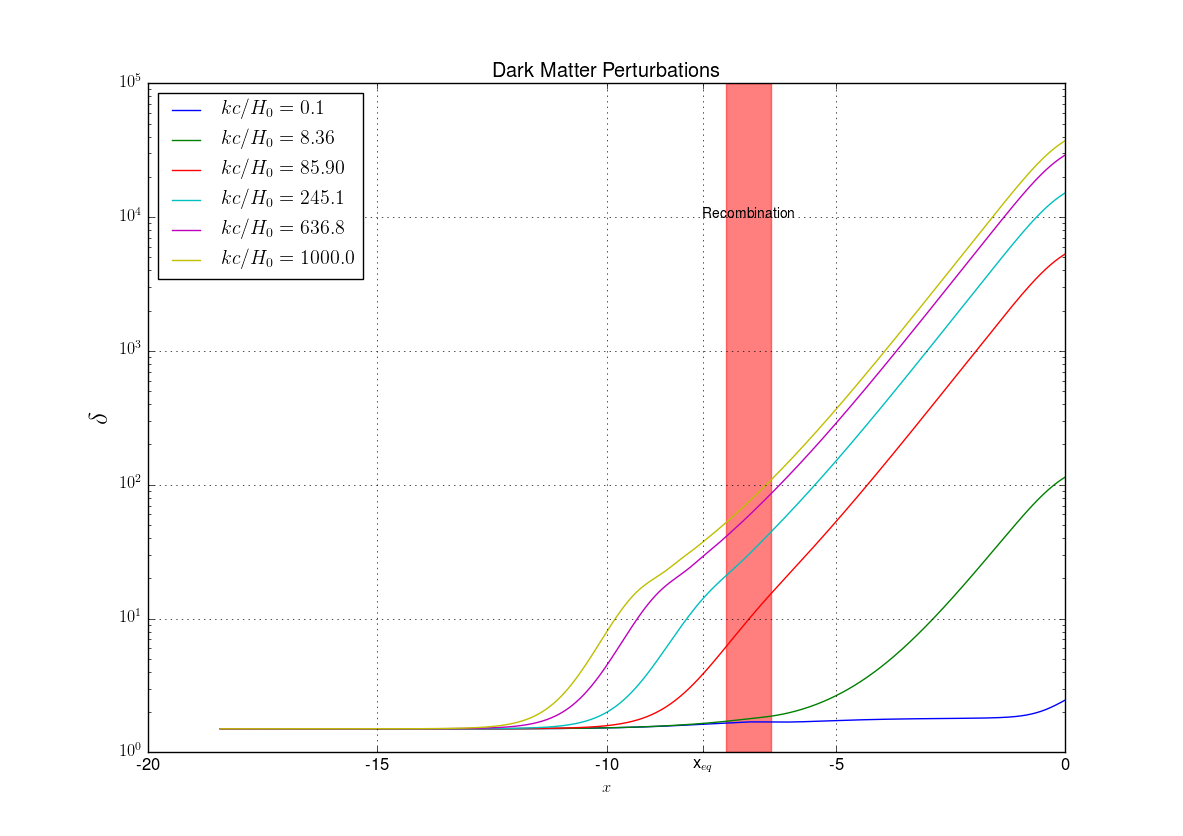
\includegraphics[width=1.0\linewidth]{delta}
\end{minipage}%
\begin{minipage}{0.5\textwidth}
\centering
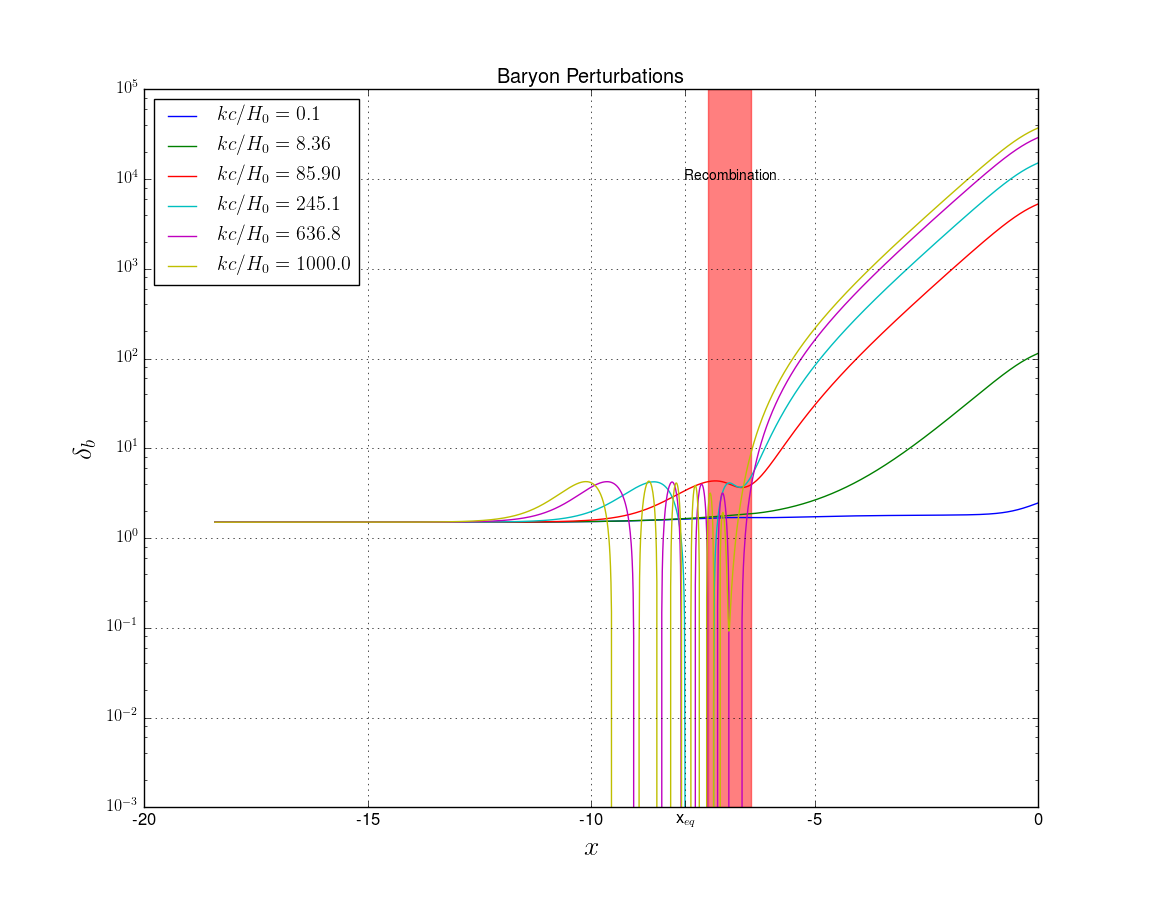
\includegraphics[width=1.0\linewidth]{delta_b}
\end{minipage}
\caption{Density perturbations of the dark matter and baryonic matter in the universe. We see that for the same scales, the perturbations of both types of matter enter the horizon at the same time. However, since dark matter is collisionless, the perturbations are not suppressed as heavily before radiation-matter equality.}
\end{figure}

\begin{figure}[ht!]
\label{fig:v}
\begin{minipage}{0.5\textwidth}
\centering
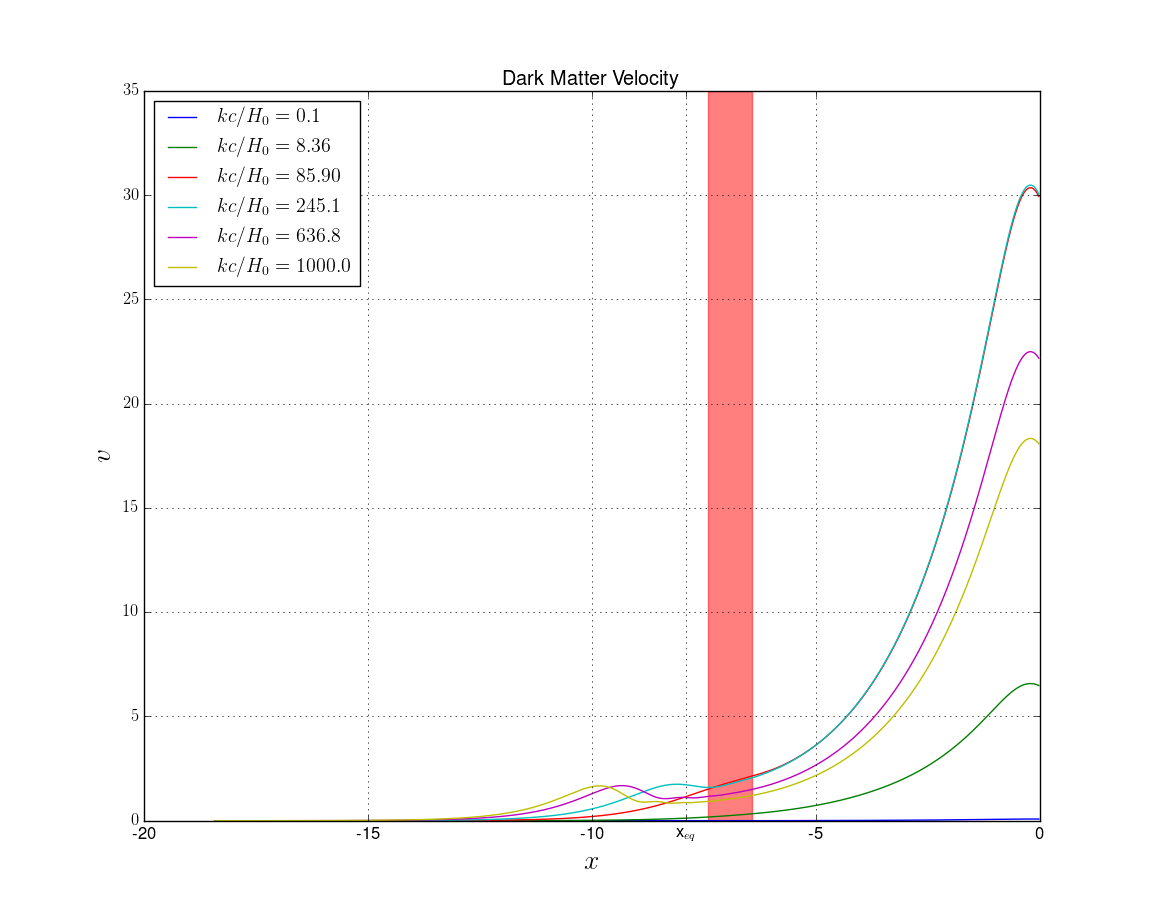
\includegraphics[width=1.0\linewidth]{v}
\end{minipage}%
\begin{minipage}{0.5\textwidth}
\centering
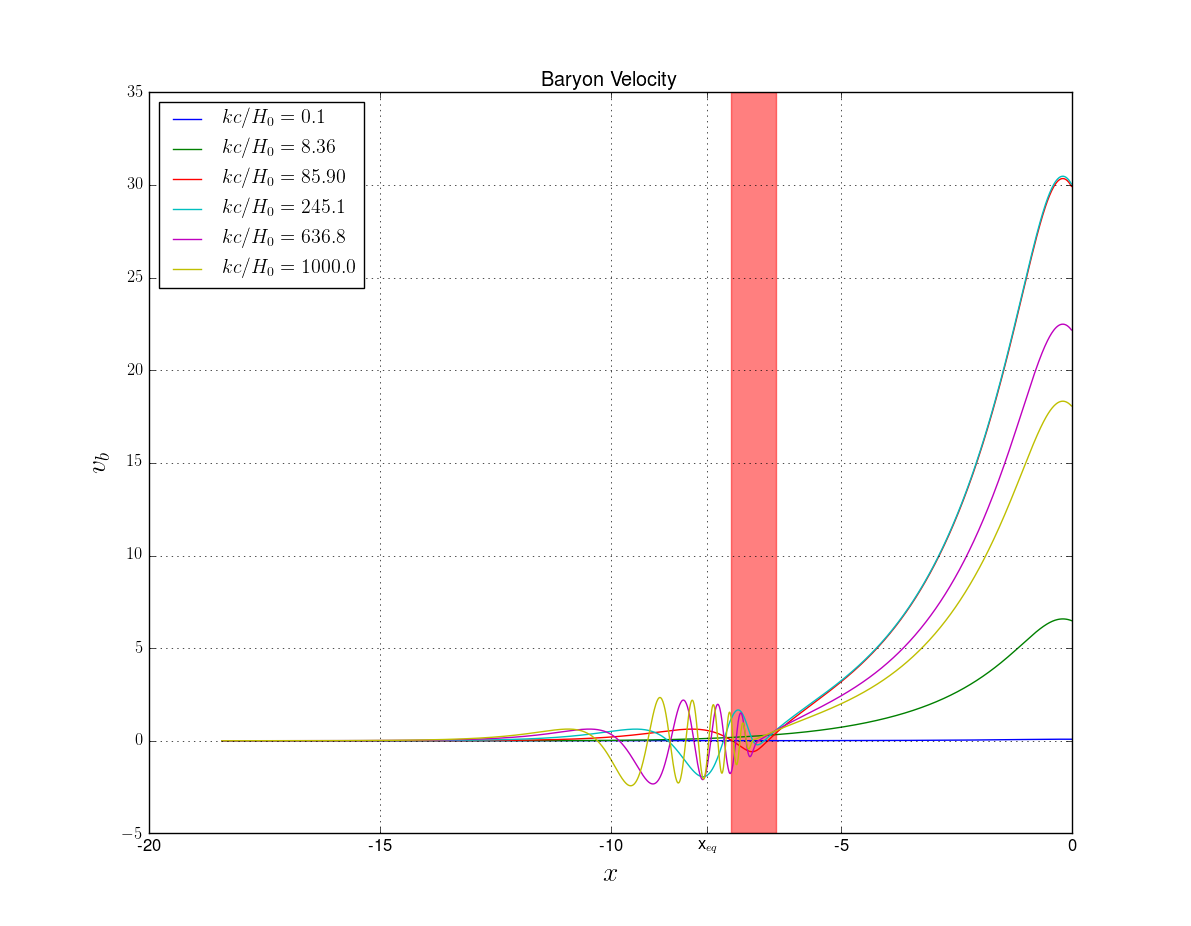
\includegraphics[width=1.0\linewidth]{v_b}
\end{minipage}
\caption{The average velocities of the dark matter and baryonic matter particles. The velocities begin to grow at the same time, and end up at the same values for $x=0$, however the behavior varies greatly before the end of recombination.}
\end{figure}

\begin{figure}[ht!]
\label{fig:pots}
\begin{minipage}{0.5\textwidth}
\centering
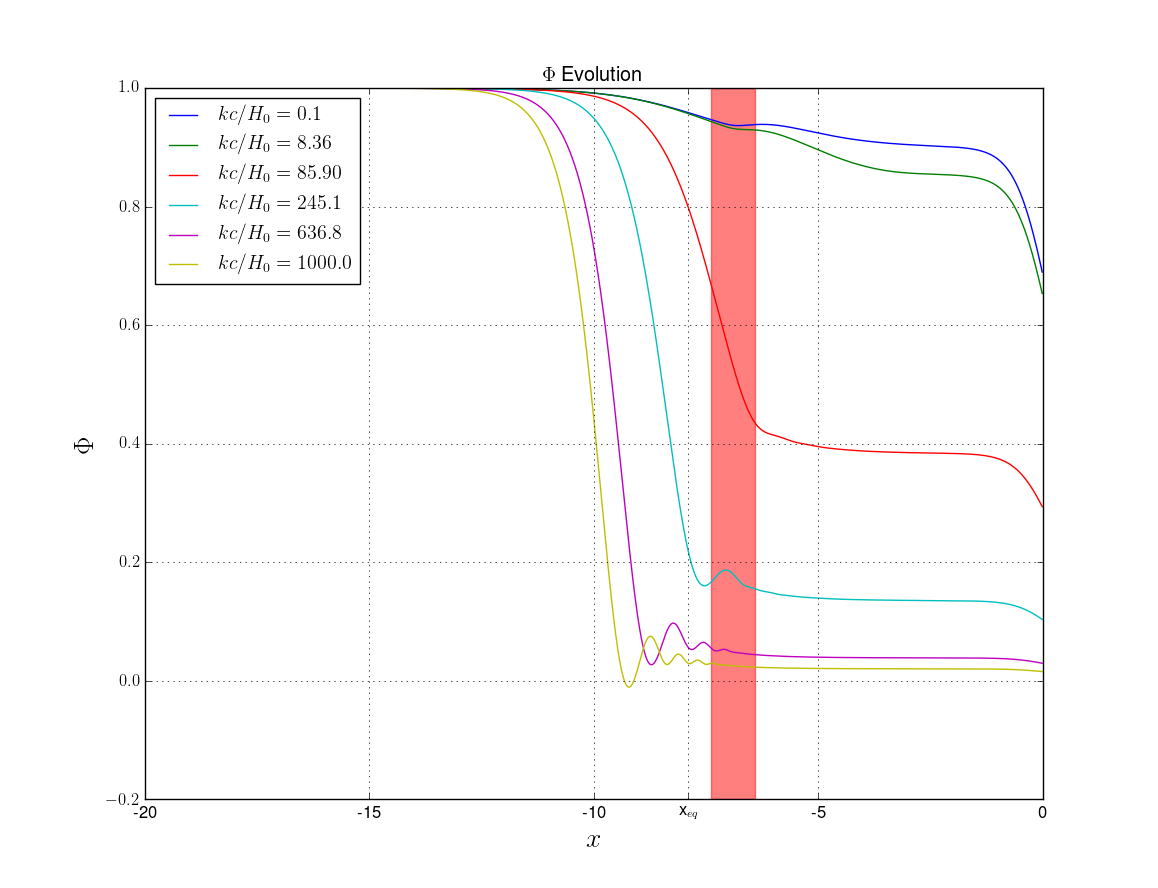
\includegraphics[width=1.0\linewidth]{phi}
\end{minipage}%
\begin{minipage}{0.5\textwidth}
\centering
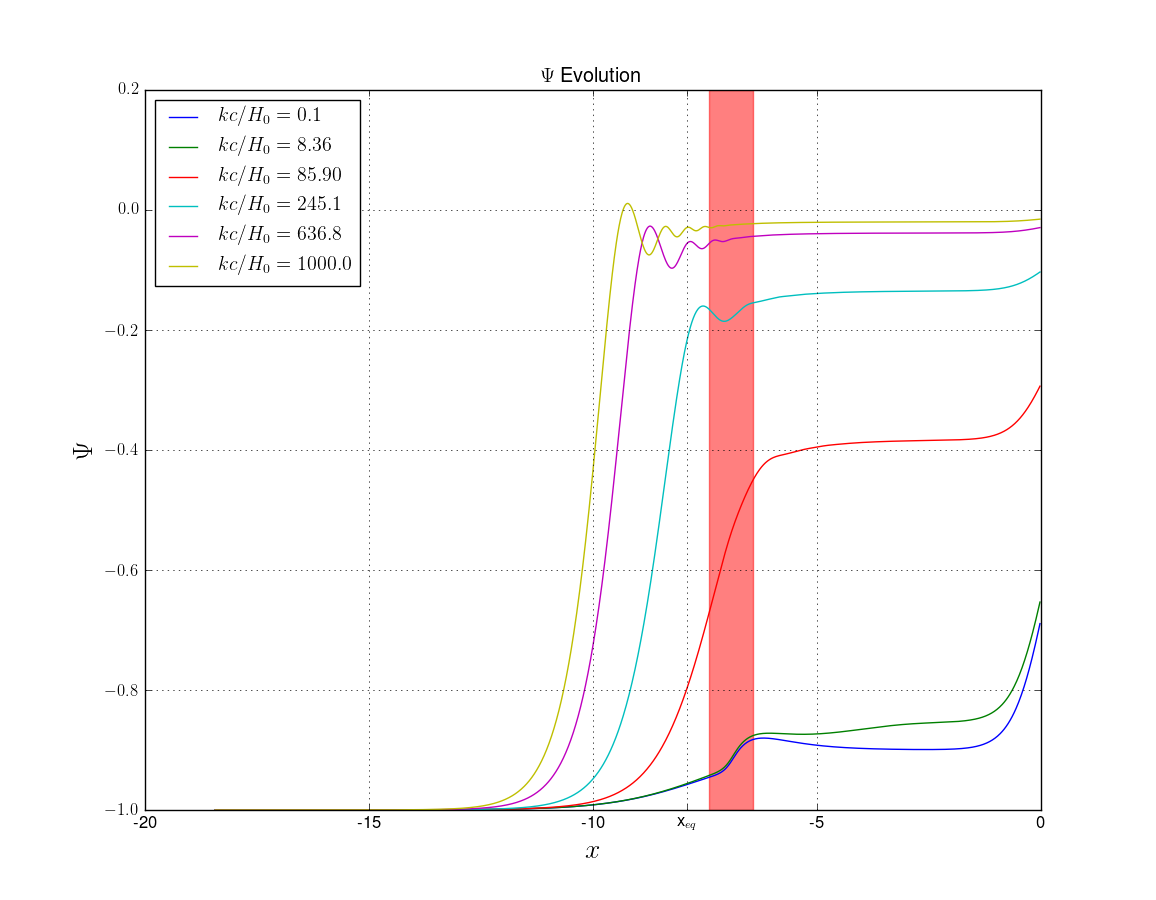
\includegraphics[width=1.0\linewidth]{psi}
\end{minipage}
\caption{Plots of the spacetime potentials $\Phi$ and $\Psi$. We showed in our derivation of the Einstein-Boltzmann equations that the two potentials counteract each other (when $\Psi$ grows, $\Phi$ decreases), which can be seen here.}
\end{figure}

\begin{figure}[ht!]
\label{fig:thetas}
\begin{minipage}{0.5\textwidth}
\centering
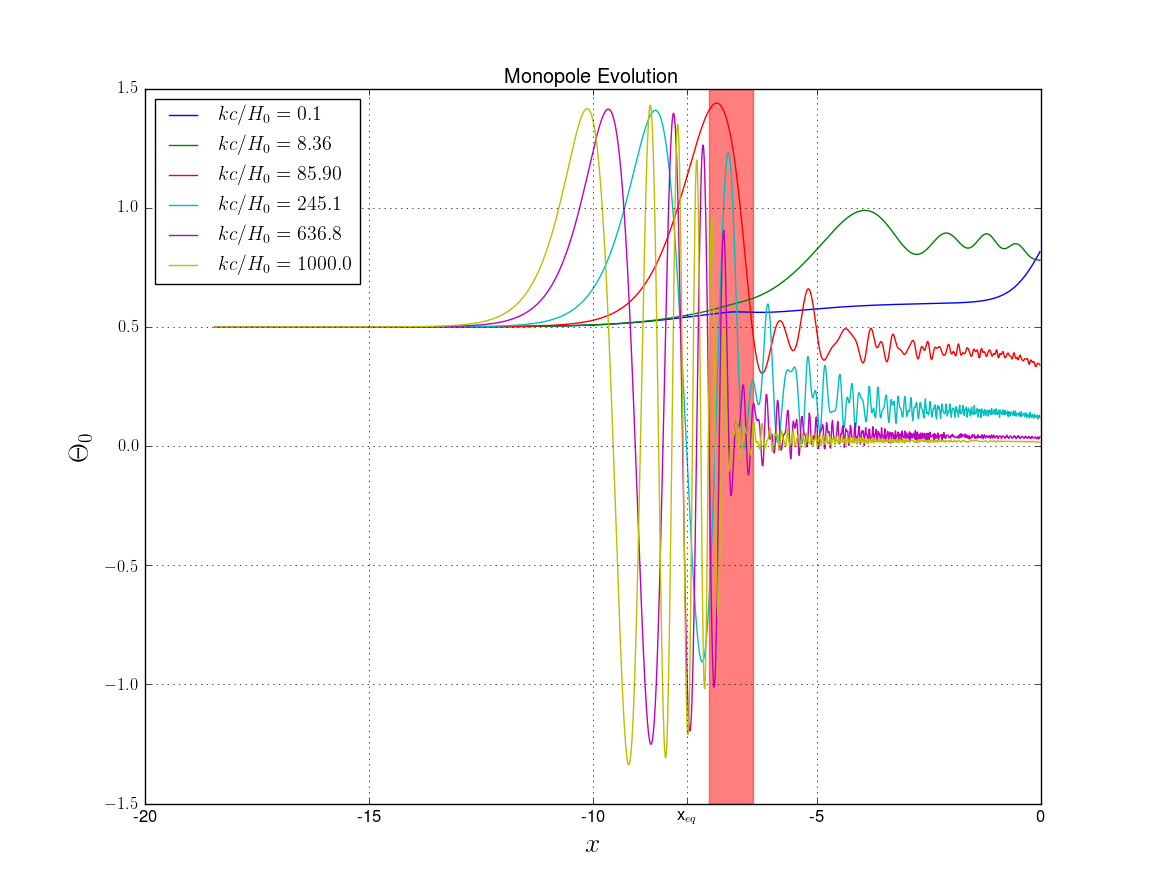
\includegraphics[width=1.0\linewidth]{theta_0}
\end{minipage}%
\begin{minipage}{0.5\textwidth}
\centering
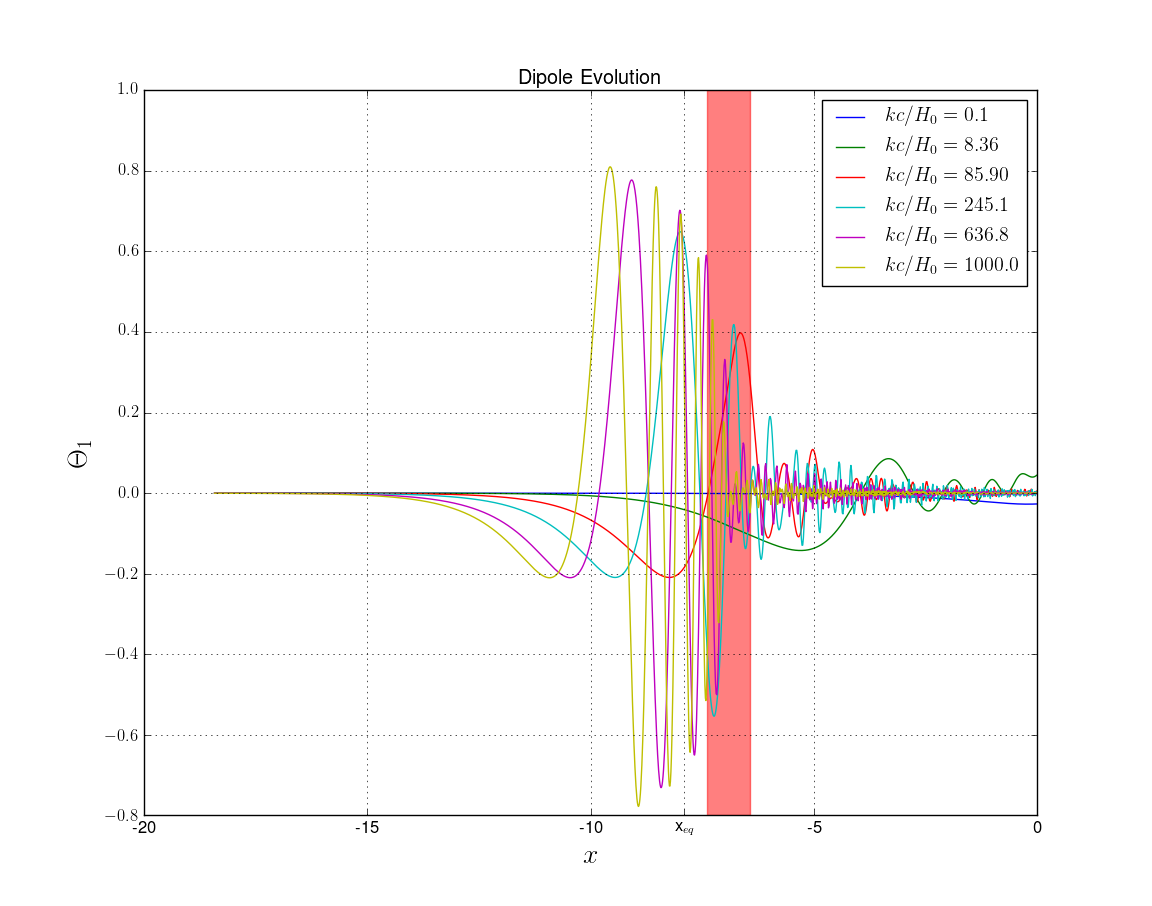
\includegraphics[width=1.0\linewidth]{theta_1}
\end{minipage}
\caption{Plots of the values of the CMB monopole and dipole values.}\end{figure}

\clearpage

\section{Discussion}\label{sec:disc}

Comparing the calculated plots to previous calculations shows that the code works as anticipated. It is important to remind the reader that small $k$ values (and therefore small $kc/H_0$) correspond to large scales, and large $k$ values correspond to small scales. By inspecting the six different $k$ values, we see a myriad of bevahiors on these varying scales. 

\subsection{Dark Matter Perturbations} 

We see in figure \ref{fig:delta} that the size of the perturbations are greater at all times once the perturbation begins to propogate from its initial scaled value of 1.5. We see that the smaller the scale we inspect, the earlier the perturbation begins to grow. We know from linear perturbation theory that the suppression of perturbations on larger scales is due to the fact that the size of the perturbations on these scales are larger than the causal horizon. We also see that the growth of the perturbation is largely independent of the size of the perturbation at any given time. This is shown by the fact that the slope of the perturbations that have entered the horizon are approximately parallel between recombination and $x \simeq -2$.\\

We know from the Einstein-Boltzmann equations that the derivatives of the perturbation growth is dependent upon the velocity of the particles. Again, by inspecting figure \ref{fig:v}, we see that for the scales that have entered the horizon, the slope of the velocities are also approximately parallel between recombination and $x \simeq -2.$ However, in this plot we see that the largest velocity does not correspond to the smallest scale. We see that the smallest scales enter the horizon earliest, and the velocities begin to increase, but are Mezaros suppressed, effectively up until the beginning of recombination when the velocities can increase again. As a result, the perturbation scales that enter the horizon closer to $x_{eq}$ end up with the highest velocities. Again, we see that the largest scales do not enter the horizon until near or after recombination and their characteristic velocities stay small. \\

\subsection{Baryon Perturbations}

The behavior of the baryon perturbations and velocities is similar to that of the dark matter in many ways. The baryonic perturbations seen in figure \ref{fig:delta} follow the same shape as the photon monopole plot in figure \ref{fig:thetas}. This is likely due to the tightly coupled nature of the photons up until near recombination for all scales. As is expected, the smallest scale perturbations enter the horizon and begin to evolve earlier, and as a result, the smallest scale perturbations become the largest after recombination.\\

The velocity of the baryonic particles seem to behave a bit more dynmamically than the dark matter particles as shown in figure \ref{fig:v}. The three smallest scales, the ones which enter the horizon the earliest oscillate around a mean value of $v_b = 0$ due to the virialization of these perturbations. Because the pressure is so high in the early universe, these virialized objects are not able to collapse completely and oscillate around their equilibrium state. The negative values of the velocity before recombinatoin correspond to the collapsing of the perturbations, while the positive values correspond to their expansion. Once recombination begins, these oscillations begin to get damped, and the baryons follow the dark matter perturbations.\\
\clearpage

\subsection{Potentials $\Phi$ and $\Psi$}

The potentials $\Phi$ and $\Psi$ correspond to the spatial and time compression and stretching of spacetime respectively. As mentioned in section \ref{subsec:init}, we scale all of our equations by setting $\Phi_{init} = 1$. We showed in lecture, that to first order we can approximate $\Psi = - \Phi$. By this we mean that a growth in $\Phi$ corresponds to a decrease in $\Psi$ and vice-versa. Although our solutions in section \ref{subsec:einbol} do not explicitly require this, we can see that the behavior of these two potentials agrees with our approximation well. For small scales, the spatial stretching of spacetime, $\Phi$, decreases quickly and maintains a value close to zero during and after recombination, while the larger scales begin to decrease their values later on. The $\Psi$ plot shows similar behavior, just reflected over the x-axis, approaching zero quickly for small scales.

\subsection{Photon Moments}

For this milestone, we only specifically look at the behavior of the first two moments of the photon perturbations in figure \ref{fig:thetas}. It is sufficient to do so because larger moments are greatly suppressed (especially before recombination), and can be determined from the values of the smaller moments. As mentioned above, the behavior of the monopole follows that of the baryon perturbations during tight coupling, and deviates afterwards. Interestingly, we see that after recombination the monopole values of the smaller scales is suppresed far more than the larger scales. I believe this is due to the evolution of the smaller scales before recombination. We see that the behavior of all scales but the largest investigated mimic a damped oscillator which goes towards $\Theta_0 = 0$. Since the smaller scales have more time to evolve, they reach values closer to zero, while the larger moments are just beginning to evolve.\\

Similarly, in the $\Theta_1$ plot, we see the dipole behavior on the smaller scales become more "quiet" shortly after recombination, while the variations in the dipole of the larger scales become more prominent.

\section{Conclusion}\label{sec:conc}

With our knowledge from Cosmology I and II we are able to recognize many behaviors theorized by modern cosmology and see some of the more physical consequences of these assumptions through this milestone. The interaction of photons and baryons plays a large role in the formation of structures on each scale. This milestone sets the stage for line of sight integration and other tools necessary to estimate the $C_l$ coefficients needed to approximate the primordial power spectrum $P(k)$. It's beneficial to see the results of actual calculations showing behaviors like Meszaros suppression.









\end{document}